\documentclass[a4paper]{article}
\usepackage{vntex}
%\usepackage[english,vietnam]{babel}
%\usepackage[utf8]{inputenc}

%\usepackage[utf8]{inputenc}
%\usepackage[francais]{babel}
\usepackage{a4wide,amssymb,epsfig,latexsym,multicol,array,hhline,fancyhdr}
\usepackage{booktabs}
\usepackage{amsmath}
\usepackage{lastpage}
\usepackage[lined,boxed,commentsnumbered]{algorithm2e}
\usepackage{enumerate}
\usepackage{color}
\usepackage{graphicx}							% Standard graphics package
\usepackage{array}
\usepackage{tabularx, caption}
\usepackage{multirow}
\usepackage[framemethod=tikz]{mdframed}% For highlighting paragraph backgrounds
\usepackage{multicol}
\usepackage{rotating}
\usepackage{graphics}
\usepackage{geometry}
\usepackage{setspace}
\usepackage{epsfig}
\usepackage{tikz}
\usepackage{listings}
\usetikzlibrary{arrows,snakes,backgrounds}
\usepackage{hyperref}
\hypersetup{urlcolor=blue,linkcolor=black,citecolor=black,colorlinks=true} 
%\usepackage{pstcol} 								% PSTricks with the standard color package

\newtheorem{theorem}{{\bf Định lý}}
\newtheorem{property}{{\bf Tính chất}}
\newtheorem{proposition}{{\bf Mệnh đề}}
\newtheorem{corollary}[proposition]{{\bf Hệ quả}}
\newtheorem{lemma}[proposition]{{\bf Bổ đề}}

\everymath{\color{blue}}
%\usepackage{fancyhdr}
\setlength{\headheight}{40pt}
\pagestyle{fancy}
\fancyhead{} % clear all header fields
\fancyhead[L]{
 \begin{tabular}{rl}
    \begin{picture}(25,15)(0,0)
    \put(0,-8){
\includegraphics[width=8mm, height=8mm]{logoITSGUsmall.png}}
    %\put(0,-8){\epsfig{width=10mm,figure=hcmut.eps}}
   \end{picture}&
	%\includegraphics[width=8mm, height=8mm]{hcmut.png} & %
	\begin{tabular}{l}
		\textbf{\bf \ttfamily Trường Đại học Sài Gòn}\\
		\textbf{\bf \ttfamily Khoa Công Nghệ Thông Tin}
	\end{tabular} 	
 \end{tabular}
}
\fancyhead[R]{
	\begin{tabular}{l}
		\tiny \bf \\
		\tiny \bf 
	\end{tabular}  }
\fancyfoot{} % clear all footer fields
\fancyfoot[L]{\scriptsize \ttfamily Bài tập lớn môn Phát triển phần mềm mã nguồn mở - Niên khóa 2023-2024}
\fancyfoot[R]{\scriptsize \ttfamily Trang {\thepage}/\pageref{LastPage}}
\renewcommand{\headrulewidth}{0.3pt}
\renewcommand{\footrulewidth}{0.3pt}


%%%
\setcounter{secnumdepth}{4}
\setcounter{tocdepth}{3}
\makeatletter
\newcounter {subsubsubsection}[subsubsection]
\renewcommand\thesubsubsubsection{\thesubsubsection .\@alph\c@subsubsubsection}
\newcommand\subsubsubsection{\@startsection{subsubsubsection}{4}{\z@}%
                                     {-3.25ex\@plus -1ex \@minus -.2ex}%
                                     {1.5ex \@plus .2ex}%
                                     {\normalfont\normalsize\bfseries}}
\newcommand*\l@subsubsubsection{\@dottedtocline{3}{10.0em}{4.1em}}
\newcommand*{\subsubsubsectionmark}[1]{}
\makeatother

\definecolor{dkgreen}{rgb}{0,0.6,0}
\definecolor{gray}{rgb}{0.5,0.5,0.5}
\definecolor{mauve}{rgb}{0.58,0,0.82}

\lstset{frame=tb,
	language=Matlab,
	aboveskip=3mm,
	belowskip=3mm,
	showstringspaces=false,
	columns=flexible,
	basicstyle={\small\ttfamily},
	numbers=none,
	numberstyle=\tiny\color{gray},
	keywordstyle=\color{blue},
	commentstyle=\color{dkgreen},
	stringstyle=\color{mauve},
	breaklines=true,
	breakatwhitespace=true,
	tabsize=3,
	numbers=left,
	stepnumber=1,
	numbersep=1pt,    
	firstnumber=1,
	numberfirstline=true
}

\begin{document}

\begin{titlepage}
\begin{center}
TRƯỜNG ĐẠI HỌC SÀI GÒN \\
KHOA CÔNG NGHỆ THÔNG TIN
\end{center}
\vspace{1cm}

\begin{figure}[h!]
\begin{center}

\includegraphics[width=3cm]{logoITSGU.png}
\end{center}
\end{figure}

\vspace{1cm}


\begin{center}
\begin{tabular}{c}
	\multicolumn{1}{l}{\textbf{{\Large PHÁT TRIỂN PHẦN MỀM MÃ NGUỒN MỞ}}}\\
	~~\\
	\hline
	\\
	\multicolumn{1}{l}{\textbf{{\Large Tên đề tài}}}\\
	\\
	
	\multicolumn{1}{l}{\textbf{{\Large Xây dựng game Tank}}}\\
	\\
	\hline
\end{tabular}
\end{center}

\vspace{3cm}

\begin{table}[h]
\begin{tabular}{rrl}
\hspace{5 cm} & GVHD: &ThS.Từ Lãng Phiêu\\
& & Nhóm 28\\
& SV: &  3120410390 - Võ Lê Trường Phát  \\
& & 3120410166 - Ngô Thanh Hiệp \\
& & 3119410471 - Lê Minh Trường \\
% & & SV3 - MSSV \\
% & & SV4 - MSSV\\
\end{tabular}
\vspace{1.5 cm}
\end{table}

\begin{center}

{\footnotesize TP. HỒ CHÍ MINH, THÁNG 5/2024}
\end{center}
\end{titlepage}


\thispagestyle{empty}

\newpage
\tableofcontents
\newpage

%%%%%%%%%%%%%%%%%%%%%%%%%%%%%%%%%


%%%%%%%%%%%%%%%%%%%%%%%%%%%%%%%%%
\section{Phần giới thiệu}
	\subsection{ Giới thiệu game Tank}

 
	Như chúng ta đã biết, hiện nay đã có rất nhiều game bắn xe tăng khác nhau, dường như trò chơi bắn xe tăng đã trở nên quá phổ biến. Để có thể đáp ứng một cách tốt nhất thị hiếu cho người chơi thì game cần phải có những tính năng ưu việt hơn các phần mềm khác.

	Chúng ta sẽ tìm hiểu về phát triển một trò chơi bắn xe tank sử dụng ngôn ngữ lập trình Python. Trò chơi này sẽ cho phép hai người chơi trên cùng một máy tính và cạnh tranh để tiêu diệt xe tank của đối thủ.

	Một trong những tính năng quan trọng của phần mềm play audio là khả năng điều khiển phát nhạc, bao gồm chức năng play, pause, stop, next, previous, shuffle, repeat... Người dùng có thể dễ dàng chọn và thay đổi các chức năng này bằng cách sử dụng các nút được hiển thị rõ ràng trên giao diện chính.


	\subsection{Chức năng của phần mềm}
	\textbf{ Các chức năng cơ bản của game tank bao gồm:}

	•	Chế độ đa người chơi: Phần mềm cho phép hai người chơi tham gia vào trò chơi cùng một máy tính. Mỗi người choi điều khiển một chiếc xe tank và mục tiêu là tiêu diệt xe tank của đối phương.

	•	Điều khiển xe tank: Người chơi có thể điều khiển chiếc xe tank của mình bằng cách sử dụng các phím mũi tên hoặc các phím điều khiển được đặt trước.

	•	Bắn và tiêu diệt đối thủ: Mục tiêu chính của trò chơi là tiêu diệt xe tank của đối thủ bằng cách sử dụng vũ khí trên xe tank của mình. Người chơi điều khiển nút bắn để nhắm chính xác vào đối thủ.

	•	Trường chiến động rất đa dạng: Trò chơi cung cấp nhiều trường chiến động đất khác nhau với các vật cản và cấu trúc để tạo ra sự thú vị và thách thức cho người chơi.

	•	Điểm số và thời gian chơi: Phần mềm ghi nhận điểm số của mỗi người chơi dựa trên số lần tiêu diệt đối thủ.

	•	Âm thanh và hiệu ứng hình ảnh: Phần mềm có âm thanh và hiệu ứng hình ảnh sống động, tạo ra một trải nghiệm chơi game độc đáo và thú vị.

	\subsection{Hướng dẫn cách chơi-Sử dụng các phím}

        Lúc vào game người chơi sẽ được chọn xe tăng mình thích. Có 2 loại xe tăng: 
        
        •	loại 1: Ở phần xe tăng này sẽ có health là 3, Speed là 5.

	•	loại 2: Ở phần xe tăng này sẽ có health là 5, Speed là 3.

        Về phần sử dụng phím để di chuyển:

	Ở người chơi 1: Sử dụng các phím W,A,S,D để di chuyển và dùng phím 1 để bắn ra những viên đạn đến đối thủ.
 
       Ở người chơi 2: Sử dụng các phím mũi tên lên xuống trái phải để di chuyển và dùng phím m để bắn ra những viên đạn đến đối thủ.

       \subsection{Cơ chế hoạt động}

    	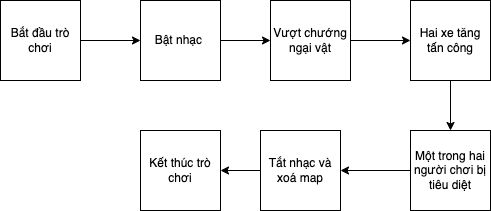
\includegraphics[width=15cm,height=10cm]{Tankhd.png}
 


\newpage
%%%%%%%%%%%%%%%%%%%%%%%%%%%%%%%%%
\section{CƠ SỞ LÝ THUYẾT}

	\subsection{Ngôn ngữ lập trình Python}

	Python là một ngôn ngữ lập trình được sử dụng rộng rãi trong các ứng dụng web, phát triển phần mềm, khoa học dữ liệu và máy học (ML). Các nhà phát triển sử dụng Python vì nó hiệu quả, dễ học và có thể chạy trên nhiều nền tảng khác nhau. Phần mềm Python được tải xuống miễn phí, tích hợp tốt với tất cả các loại hệ thống và tăng tốc độ phát triển.

	Những lợi ích của Python bao gồm:

	•	Các nhà phát triển có thể dễ dàng đọc và hiểu một chương trình Python vì ngôn ngữ này có cú pháp cơ bản giống tiếng Anh. 

	•	Python giúp cải thiện năng suất làm việc của các nhà phát triển vì so với những ngôn ngữ khác, họ có thể sử dụng ít dòng mã hơn để viết một chương trình Python.

	•	Python có một thư viện tiêu chuẩn lớn, chứa nhiều dòng mã có thể tái sử dụng cho hầu hết mọi tác vụ. Nhờ đó, các nhà phát triển sẽ không cần phải viết mã từ đầu.

	•	Các nhà phát triển có thể dễ dàng sử dụng Python với các ngôn ngữ lập trình phổ biến khác như Java, C và C++.

	•	Cộng đồng Python tích cực hoạt động bao gồm hàng triệu nhà phát triển nhiệt tình hỗ trợ trên toàn thế giới. Nếu gặp phải vấn đề, bạn sẽ có thể nhận được sự hỗ trợ nhanh chóng từ cộng đồng.

	•	Trên Internet có rất nhiều tài nguyên hữu ích nếu bạn muốn học Python. Ví dụ: bạn có thể dễ dàng tìm thấy video, chỉ dẫn, tài liệu và hướng dẫn dành cho nhà phát triển.

	•	Python có thể được sử dụng trên nhiều hệ điều hành máy tính khác nhau, chẳng hạn như Windows, macOS, Linux và Unix.

	\subsection{Phần mềm lập trình Visual Studio Code}
	
	Visual Studio Code chính là ứng dụng cho phép biên tập, soạn thảo các đoạn code để hỗ trợ trong quá trình thực hiện xây dựng, thiết kế website một cách nhanh chóng. Visual Studio Code hay còn được viết tắt là VS Code. Trình soạn thảo này vận hành mượt mà trên các nền tảng như Windows, macOS, Linux. Hơn thế nữa, VS Code còn cho khả năng tương thích với những thiết bị máy tính có cấu hình tầm trung vẫn có thể sử dụng dễ dàng.

	Visual Studio Code mang rất nhiều ưu điểm vượt trội so với bất kỳ IDE nào khác:

	•	Hỗ trợ đa nền tảng: Linux, Mac, Windows, ...

	•	Hỗ trợ đa ngôn ngữ: C/C++, JavaScript, JSON, Visual Basic, HTML, CSS, ...

	•	Ít dung lượng

	•	Tính năng mạnh mẽ

	•	Intellisense chuyên nghiệp

	•	Giao diện thân thiện

	•	Kiến trúc mạnh mẽ và người dùng có thể khai thác mở rộng

	•	Số lượng người sử dụng lớn tạo nên cộng đồng hỗ trợ rộng rãi

	

	\subsection{Thư viện hỗ trợ}
	\textbf{ Thư viện Pygame}

	Pygame là một thư viện mã nguồn mở cho phép lập trình game và đa phương tiện trên Python. Thư viện này cung cấp các công cụ cho việc tạo các ứng dụng đa phương tiện, chẳng hạn như các trò chơi, âm nhạc, đồ họa và các ứng dụng tương tự.

	Ưu điểm của Pygame:

	•	Dễ học: Pygame có cú pháp đơn giản và dễ hiểu, cho phép người dùng mới bắt đầu nhanh chóng học được cách sử dụng thư viện.

	•	Đa nền tảng: Pygame có thể hoạt động trên nhiều nền tảng khác nhau, bao gồm Windows, Mac OS X, Linux và nhiều hệ điều hành khác.

	•	Đa dạng: Pygame có nhiều tính năng và hỗ trợ đầy đủ cho các yêu cầu phức tạp trong lập trình game và đa phương tiện.

	•	Cộng đồng lớn: Pygame có một cộng đồng lớn với nhiều tài liệu hướng dẫn và các ví dụ, giúp người dùng tìm hiểu và giải quyết các vấn đề.

	Nhược điểm của Pygame:

	•	Khả năng tối ưu hóa không tốt: Pygame không được tối ưu hóa tốt cho các ứng dụng có đồ họa phức tạp, do đó, nếu không được xử lý tốt, có thể dẫn đến giảm hiệu suất.

	•	Hạn chế đồ họa: Pygame không hỗ trợ các tính năng đồ họa cao cấp như DirectX hay OpenGL, vì vậy không thể sử dụng để tạo ra các trò chơi và ứng dụng đồ họa cao cấp.

	•	Không được bảo trì thường xuyên: Pygame không được bảo trì và cập nhật thường xuyên, do đó, có thể không hoạt động tốt với các phiên bản Python mới nhất.

	•	Không hỗ trợ 3D: Pygame không hỗ trợ lập trình 3D, do đó không phù hợp để tạo ra các trò chơi và ứng dụng có đồ họa 3D phức tạp.
	
	
\newpage
\section{Thiết kế ứng dụng}
	\subsection{Ý tưởng trò chơi}
	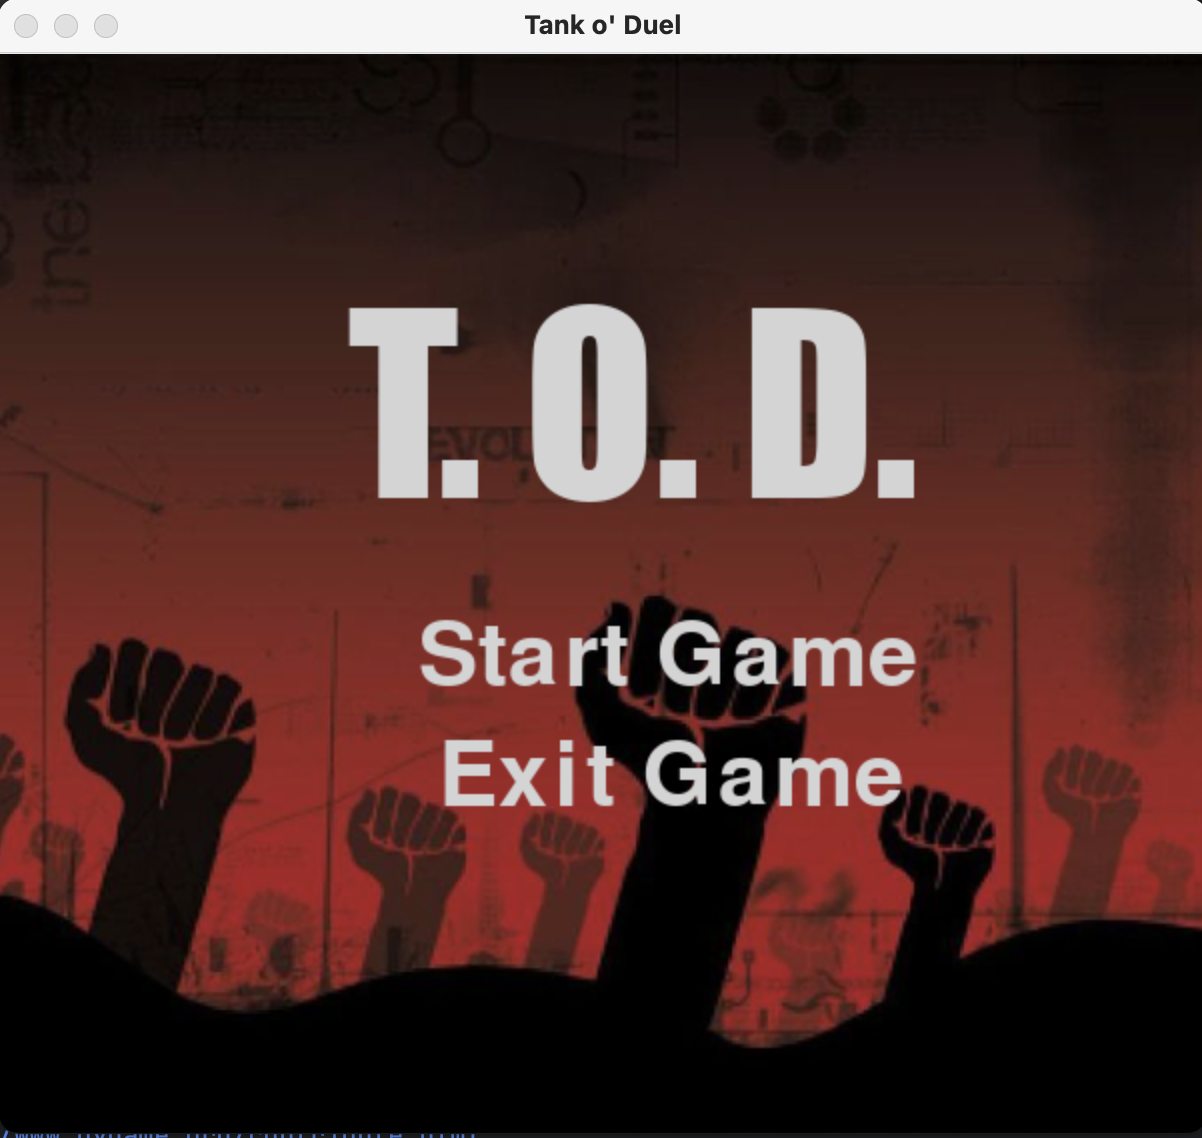
\includegraphics[width=15cm,height=10cm]{maingame.png}

	Trò chơi bắt đầu bằng việc import thư viện pygame, khởi động Pygame, thiết lập Pygame Mixer cho âm thanh, khởi tạo màu sắc và biến font. Sau đó, tạo cửa sổ trò chơi, thiết kế hình nền, nạp âm thanh, hình ảnh bản đồ và xe tăng, đặt điểm xuất hiện xe tăng, tạo nhóm người chơi, nhân vật, thêm xe tăng, quản lý tường và viên đạn, và cuối cùng đặt biến điều khiển cho hàm và vòng lặp trong trò chơi.

        Ghi điểm vào file điểm khi có, thiết lập số khung hình trên giây để chạy mượt mà, gọi hàm menu để hiển thị giao diện người chơi và xử lý sự kiện chuột. Khi người dùng chọn "chơi trò chơi", hàm menu sẽ kết thúc và dừng phát nhạc nền. Khi chọn "thoát trò chơi", hàm menu sẽ kết thúc, đặt giá trị false cho biến điều khiển và dừng phát nhạc.

        Nhóm tải và phát nhạc nền khi call màn hình lựa chọn xe tăng, hiển thị tên các mục lựa chọn và hình ảnh, yêu cầu người chơi sử dụng phím điều khiển để chuyển đổi xe tăng. Khi người chơi nhấn Enter, xác nhận xe tăng được chọn và cập nhật thông số. Sau đó, chọn bản đồ và kết thúc hàm lựa chọn. Nếu người chơi thoát, hàm sẽ kết thúc và dừng phát nhạc.
        
        Nhóm hẹn giờ cho việc bắn đạn khi màn hình chiến đấu được kích hoạt, sau đó nạp và phát nhạc nền. Trong vòng lặp, họ di chuyển người chơi, xử lý việc bắn đạn và đóng cửa sổ trò chơi. Duyệt qua đạn để xử lý va chạm và hiển thị trạng thái trên màn hình. Khi sức khỏe của người chơi giảm về 0, kết thúc trò chơi và dừng nhạc nền.
        
        Nhóm sẽ tải và phát nhạc nền khi hàm kết thúc trò chơi được gọi, sau đó cập nhật điểm số từ tệp và xác định người chiến thắng. Người chiến thắng sẽ được cộng thêm một điểm và điểm số mới sẽ được ghi lại. Tiêu đề kết quả sẽ được hiển thị trên màn hình và trong vòng lặp, điểm số sẽ được hiển thị và xử lý sự kiện như dừng phát nhạc, thiết lập lại điểm số hoặc kết thúc trò chơi sẽ được thực hiện.
            
        Tạo ra một vùng trống bị giới hạn bởi rìa bản đồ, sau đó thiết lập hai đối thủ (ta và địch), mỗi đối tượng sẽ đặt ở 2 góc bản đồ. Đưa xe tăng của hai người chơi lên bản đồ, player 1 đặt ở góc trái bên trên map, player 2 đặt ở góc dưới bên phải map.

        Sau đó 2 chiếc xe tăng sẽ đối đầu lẫn nhau bằng cách bắn đạn nhằm hạ gục đối phương, đồng thời cố gắng di chuyển để né đạn từ địch.
        
        Để tạo ra một trải nxuấtệm chơi đầy sinh động và hấp dẫn hơn, nhóm em sẽ thiết kế các vách tường gỗ đặc biệt, những bức tường chắn đạn sẽ ngăn cản việc bắn trực tiếp vào nhau. Điều này sẽ tạo ra các tình huống chiến đấu trong game trở nên chân thực hơn, khi người chơi phải tìm cách vượt qua các vách tường này để tiến xa hơn trong trận đấu

	\subsection{Sử dụng thư viện}

        Các thư viện được sử dụng:

        import Math 
        
        import pygame from pygame.locals import * 
        
        import random
        
        import time
        
        pygame.init()

        - Math: Thư viện toán học chuẩn của Python, cung cấp các hàm toán học như lũy thừa, căn bậc hai, các hàm lượng giác.

        - pygame: Thư viện chuyên cho việc phát triển trò chơi, hỗ trợ tạo cửa sổ, xử lý đồ họa, âm thanh, và xử lý sự kiện.
    
        - from pygame.locals import : Nhập tất cả các hằng số có sẵn từ module pygame.locals, thường được sử dụng để dễ dàng tham chiếu tới các nút bấm, hằng số hệ thống mà không cần phải gọi module pygame.locals.

        - random: Thư viện hỗ trợ tạo ra các số ngẫu nhiên, sử dụng cho việc lựa chọn ngẫu nhiên, xáo trộn dữ liệu.

        - time: Thư viện cung cấp các hàm để làm việc với thời gian, bao gồm đo hạn, đợi (sleep), và xuất lại thời gian hệ thống

        - pygame.init(), thư viện pygame được khởi tạo, đây là bước cần thiết để bắt đầu làm việc với pygame.



	\subsection{Thực hiện trò chơi }
	\textbf{*Khởi tạo menu:}
 
        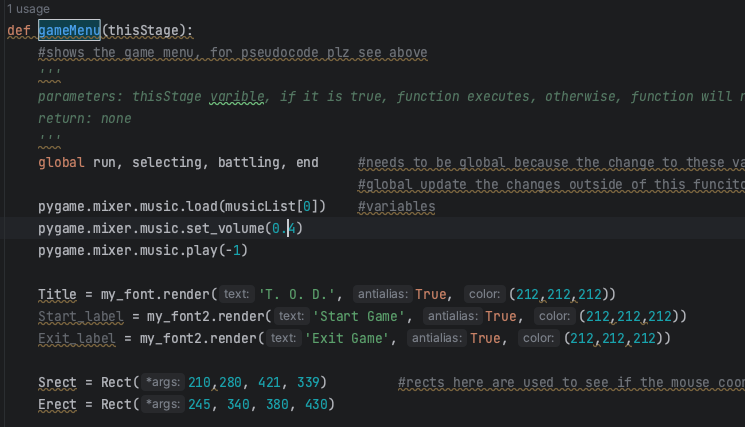
\includegraphics[width=15cm,height=10cm]{imgcodemenu.png}

        function gameMenu trong ứng dụng Pygame có vai trò thiết lập màn hình menu chính cho trò chơi. Ở trung tâm của hàm gameMenu là tham số thisStage, cho phép xác định các giai đoạn hoặc trạng thái cụ thể trong giao diện menu. Tham số này phục vụ như một yếu tố linh hoạt thích ứng với tương tác của người dùng, hướng dẫn họ qua menu một cách mượt mà.

        Việc khai báo các biến toàn cục như run, selecting, battling và end cung cấp cho hàm sự linh hoạt để sửa đổi các giá trị này trong quá trình thực thi. Những biến này hoạt động như các cờ kiểm soát, ảnh hưởng đến hành vi của menu dựa trên đầu vào của người dùng và sự kiện hệ thống.

        \textbf{*Sự kiện thoát game}

         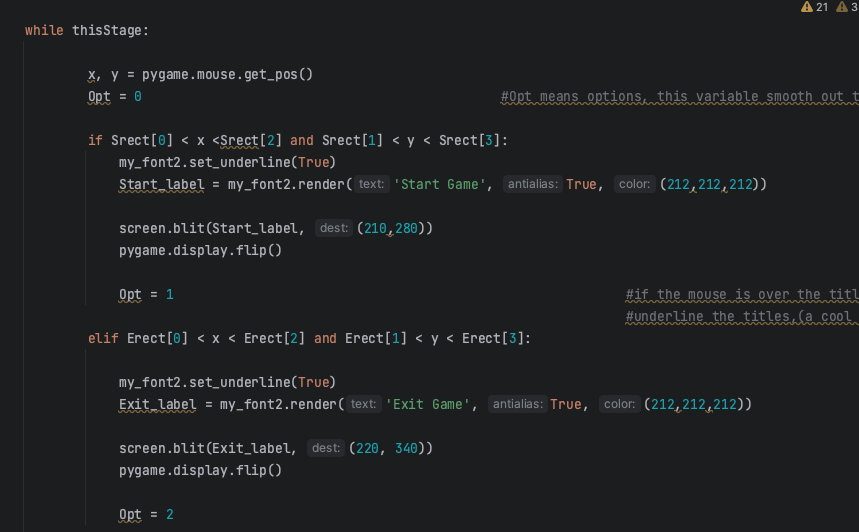
\includegraphics[width=15cm,height=10cm]{imgcodeendgame.png}
         
         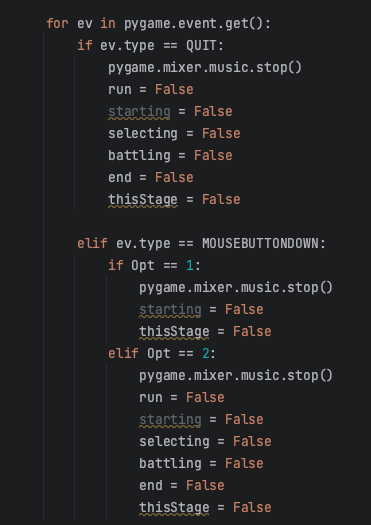
\includegraphics[width=15cm,height=10cm]{imgcodeendgame2.png}

        Thiết lập của vòng lặp cho menu trò chơi. Quản lý việc hiển thị và tương tác của người dùng với menu chính, xử lý việc bắt đầu hay thoát trò chơi dựa trên đầu vào từ chuột. Trong vòng lặp while này, các sự kiện chuột và tương tác người dùng được xử lý:

        - Hàm pygame.mouse.get_pos() lấy vị trí hiện tại của con trỏ chuột.
        
        - Opt được khởi tạo với giá trị 0, có thể được sử dụng để theo dõi lựa chọn của người chơi trong menu.
        
        - if Srect[0] < x < Srect[2] and Srect[1] < y < Srect[3]: kiểm tra nếu con trỏ chuột đang ở bên trên nút "Start Game". Nếu đúng, thì chữ "Start Game" được gắn dấu gạch dưới.

        - elif Erect[0] < x < Erect[2] and Erect[1] < y < Erect[3]: thực hiện việc kiểm tra tương tự cho nút "Exit Game". Nếu đúng, thì chữ "Exit Game" được in đậm và màu đỏ, được thể hiện bằng nhãn Exit_label. Biến Opt được thiết lập là 2.

        \textbf{*Thiết lập màn hình chọn xe tăng}
        
        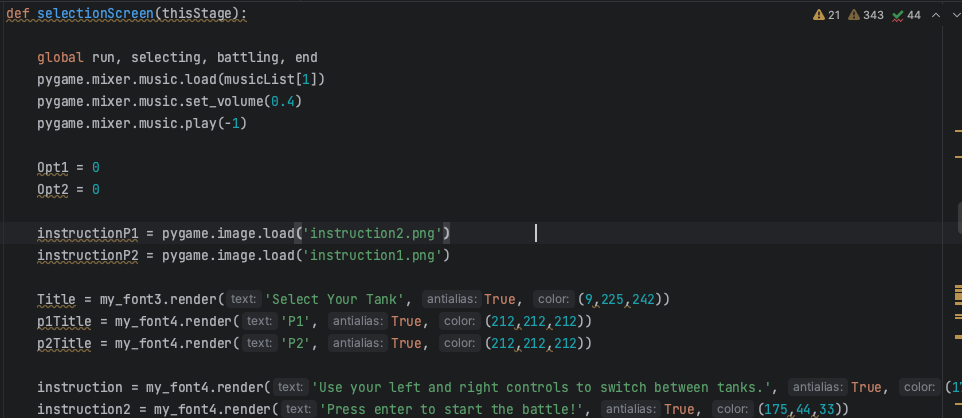
\includegraphics[width=12cm,height=7cm]{selecteTank.png}

        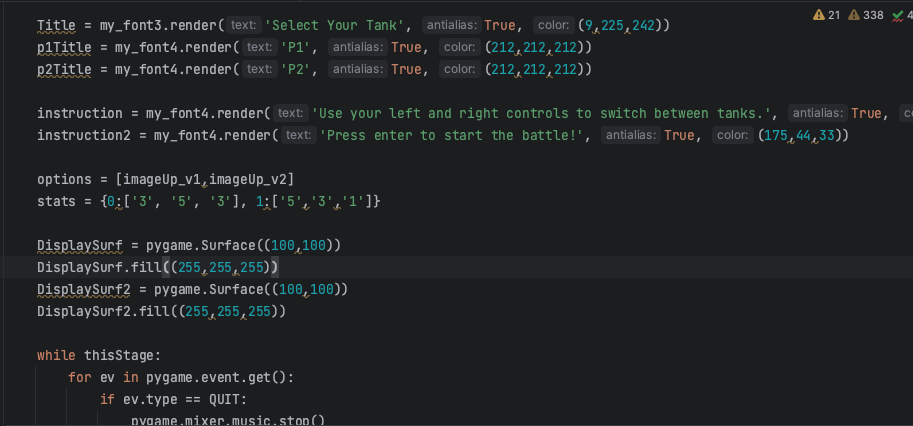
\includegraphics[width=12cm,height=7cm]{selectedTank2.png}

        Quản lý quá trình chọn xe tăng và cài đặt các thông số trước khi bắt đầu trò chơi. Lựa chọn và thao tác được thực hiện thông qua các phím điều hướng và phím ENTER. Hàm này xử lý màn hình lựa chọn xe tăng trước khi bắt đầu trận chiến.

        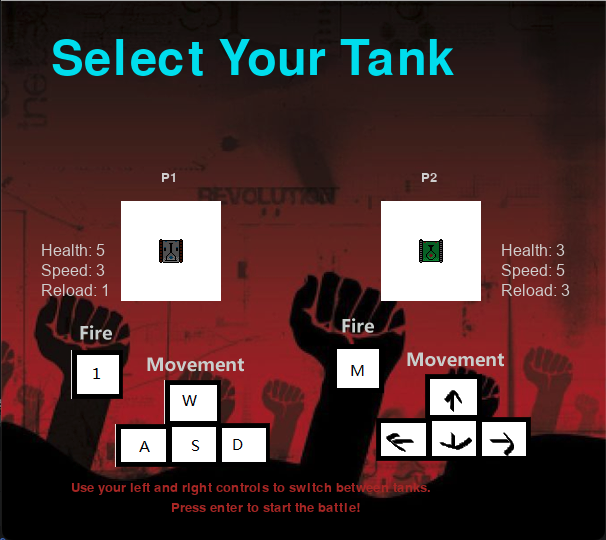
\includegraphics[width=12cm,height=7cm]{selectedTank3.png}

        Ta thiết lập biến toàn cục gồm run, selecting, battling, và end. Hàm tải và phát nhạc nền từ musicList[1] với âm lượng đã được đặt là 0.4 và lặp lại vô hạn.

        \textbf{*Thiết lập định dạng cho xe tăng}

        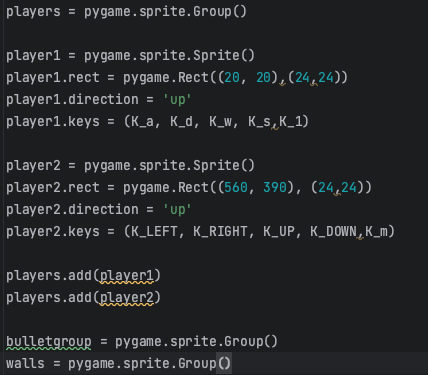
\includegraphics[width=12cm,height=7cm]{positiontank.png}

        - Khai báo hai danh sách ver1 và ver2 chứa các hình ảnh khác nhau cho hai phiên bản người chơi, với các hướng di chuyển khác nhau được biểu diễn qua các hình ảnh lên, xuống, phải và trái.

        - Tạo nhóm players sử dụng pygame.sprite.Group() để quản lý các đối tượng người chơi.
        
        - Tạo ra hai đối tượng player1 và player2 bằng cách sử dụng pygame.sprite.Sprite(). Mỗi đối tượng người chơi được cấp một hình chữ nhật (rect) để xác định vị trí và kích thước, một thuộc tính direction để biết hướng di chuyển, và một set các keys để xác định các phím điều khiển di chuyển và bắn đạn.
        
        - Thêm hai đối tượng player1 và player2 vào nhóm players bằng phương thức add.

        - Nhóm bulletgroup sử dụng pygame.sprite.Group(), dùng để quản lý các viên đạn trong trò chơi.
        
        - Nhóm walls cũng dùng pygame.sprite.Group(), dùng để quản lý các bức tường trong game.

        \textbf{*Cách thức hoạt động điều khiển xe tăng}

         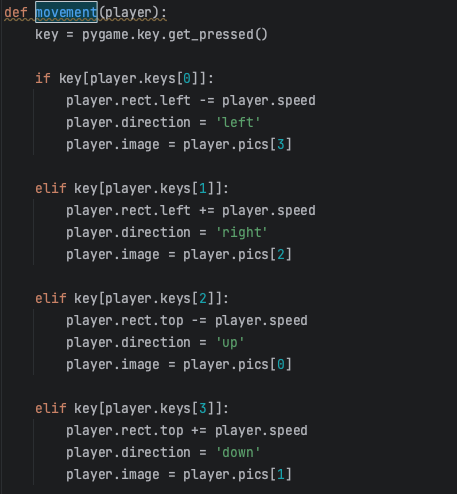
\includegraphics[width=12cm,height=7cm]{movetank1.png}

         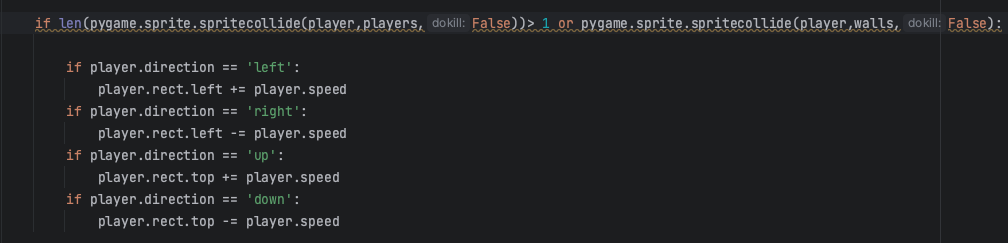
\includegraphics[width=15cm,height=7cm]{movetank2.png}

         - Hàm movement nhận đối tượng player làm đối số và xử lý các sự kiện đầu vào từ bàn phím để di chuyển player.
         
        - Hàm sử dụng biến key để lấy trạng thái hiện tại của các phím được bấm.
        
        - Mỗi phím kiểm soát một hướng di chuyển cụ thể của player (sang trái, sang phải, lên trên, xuống dưới) và cập nhật hình ảnh player tương ứng với hướng đó.
            
        - Hàm cũng xử lý va chạm để ngăn player không di chuyển xuyên qua các đối tượng khác như người chơi hoặc tường:
        + Sử dụng pygame.sprite.spritecollide để kiểm tra va chạm giữa player và nhóm players hoặc walls.

        + Nếu phát hiện va chạm len() của danh sách va chạm lớn hơn 1 hoặc spritecollide trả về True, player sẽ phải di chuyển theo hướng ngược lại để tránh tình trạng mắc kẹt.
        
        +Đối với mỗi hướng di chuyển, nếu phát hiện va chạm, player sẽ được đẩy ngược lại một khoảng bằng player.speed để không đè lên player khác hoặc các bức tường trong trò chơi.

        \textbf{*Tạo map}

        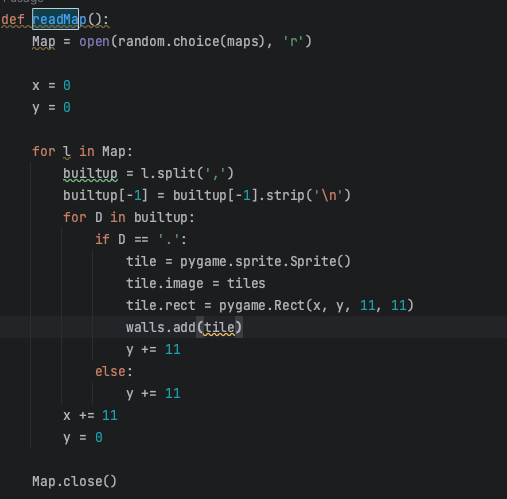
\includegraphics[width=12cm,height=7cm]{readmap.png}

        Hàm readMap được tạo ra để đọc dữ liệu từ bản đồ của trò chơi và thiết lập màn hình chơi dựa theo nó, sử dụng sprites để tạo ra các đối tượng "bức tường", và đặt chúng vào vị trí tương ứng trên màn hình chơi của trò chơi.

        Lệnh open mở tệp, và random.choice chọn một tệp một cách ngẫu nhiên từ danh sách đó. Hai biến x và y được khởi tạo để theo dõi vị trí hiện tại trên bản đồ, nơi các đối tượng của trò chơi sẽ được đặt.
        
        Sau đó duyệt qua từng dòng của tệp bản đồ (for l in Map):
        
        - Mỗi dòng được chia (split) bởi dấu phẩy để tạo thành một danh sách các ký tự, mỗi ký tự đại diện cho một phần của bản đồ.
        
        - Hàm loại bỏ ký tự xuống dòng n ở cuối mỗi dòng (builtup[-1] = builtup[-1].strip('n')).
        
        Tiếp theo, hàm duyệt qua từng ký tự trong dòng (for D in builtup):
        
        - Nếu ký tự là dấu chấm (.), nó tượng trưng cho một "bức tường" trong trò chơi:
        
        - Một đối tượng sprite mới được tạo ra (tile = pygame.sprite.Sprite()).
        
        - Ảnh đại diện cho bức tường, biến tiles, được thiết lập làm hình ảnh của sprite này (tile.image = tiles).
        
        - Đối tượng sprite mới đó được gán một hình chữ nhật (Rect) với vị trí (x, y) và kích thước (12, 12).

        - Đối tượng sprite được thêm vào nhóm walls, đã được định nghĩa trước đây như một nhóm của spritesPygame, để dễ dàng quản lý các bức tường trong trò chơi.
    
        - y được tăng thêm 12 để di chuyển đến vị trí tiếp theo trên cùng một dòng, nơi một sprite khác được đặt.
        
        - Nếu ký tự không phải là dấu chấm, y vẫn được tăng lên và không có sprite nào được tạo ra.
        
         \textbf{*Xử lý màn hình trận đấu}

         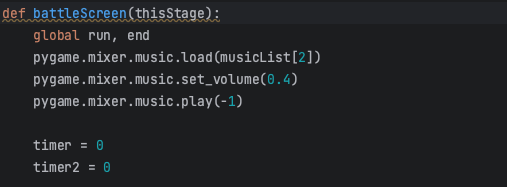
\includegraphics[width=12cm,height=7cm]{battleSreen.png}

         Thiết lập và quản lý màn hình chiến đấu trong game, bao gồm việc khởi tạo âm nhạc và điều chỉnh âm lượng, bắt đầu vòng lập, và khởi tạo bộ đếm thời gian cho các sự kiện trong trò chơi.

        \textbf{*Xử lý bắn đạn }
        
        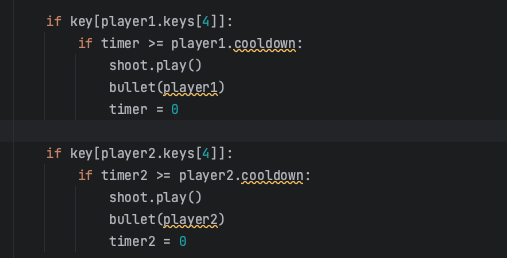
\includegraphics[width=12cm,height=7cm]{firetank.png}

        Quản lý việc bắn đạn cho hai người chơi trong trò chơi. Khi người chơi nhấn nút bắn đạn (được chỉ định bởi player1.keys[4] và player2.keys[4]), và nếu thời gian đếm đã đủ lớn so với khoảng thời gian hồi chiêu (cooldown), âm thanh bắn đạn sẽ được phát, một viên đạn mới sẽ được tạo từ vị trí của người chơi đó, và bộ đếm thời gian sau đó sẽ được đặt lại về 0 để bắt đầu đếm cho lần bắn tiếp theo.

         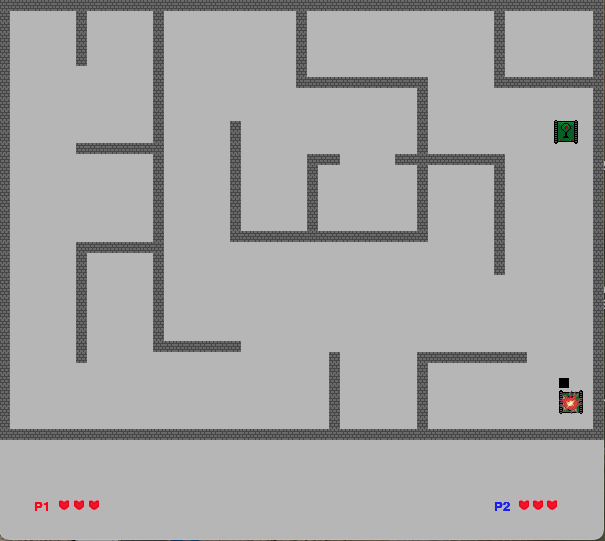
\includegraphics[width=12cm,height=7cm]{imgfiretank2.png}

        \textbf{*Kiểm tra tank nổ khi trúng đạn }
        
        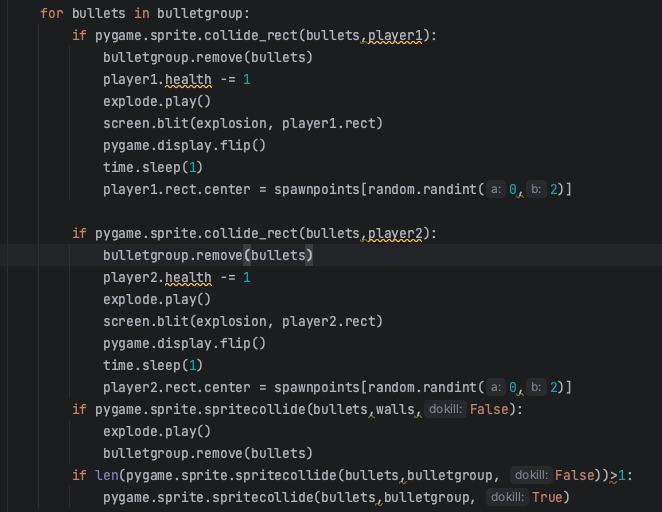
\includegraphics[width=12cm,height=7cm]{wartank.png}

        Xử lý va chạm của đạn với các nhân vật trong trò chơi và các đối tượng khác nhau trên màn hình. Khi một viên đạn từ bulletgroup va chạm vào người chơi player1 hoặc player2, viên đạn đó sẽ bị loại bỏ khỏi nhóm, người chơi sẽ mất một lượng máu, âm thanh nổ sẽ được phát và một hình ảnh vụ nổ sẽ xuất hiện tại vị trí của người chơi. Người chơi sau đó sẽ được chuyển đến điểm spawn xa nhất so với vị trí hiện tại của người chơi kia. Nếu viên đạn va chạm vào tường, nó cũng sẽ bị loại bỏ và phát ra âm thanh nổ.

        Nếu có nhiều viên đạn va chạm vào nhau (được kiểm tra bởi len(pygame.sprite.spritecollide(bullets,bulletgroup, False))>1), tất cả những viên đạn va chạm sẽ được loại bỏ.

        \textbf{*Kết thúc ván đấu }

        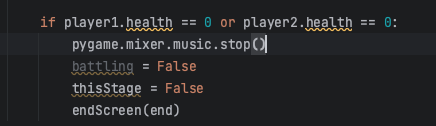
\includegraphics[width=12cm,height=7cm]{endWar.png}

        Âm nhạc trong trò chơi sẽ dừng lại sử dụng pygame.mixer.music.stop()
        
         Quản lý việc kết thúc trận đấu khi một người chơi đã mất hết health và quá trình dọn dẹp liên quan sau trận đấu, xử lý tình huống nếu một trong hai người chơi hết máu (health bằng 0). Khi một người chơi hết máu

         \textbf{*Hiển thị kết quả }

         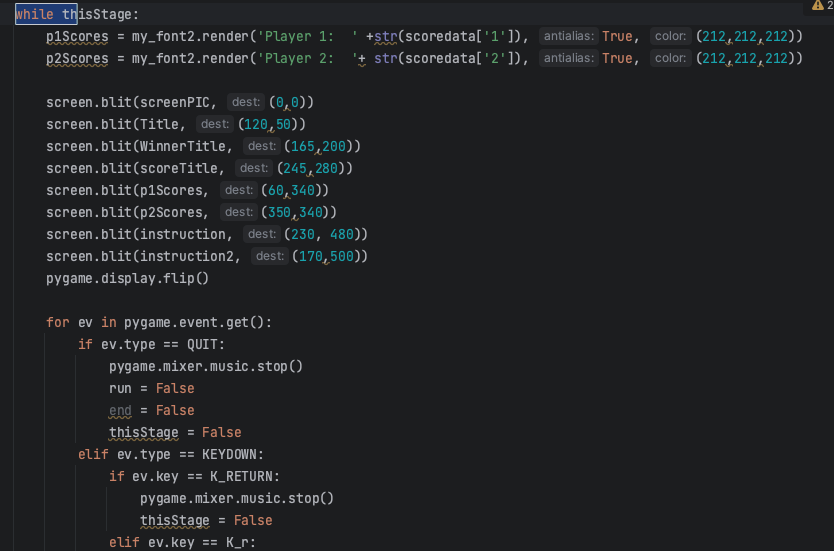
\includegraphics[width=12cm,height=7cm]{kq1.png}
         
         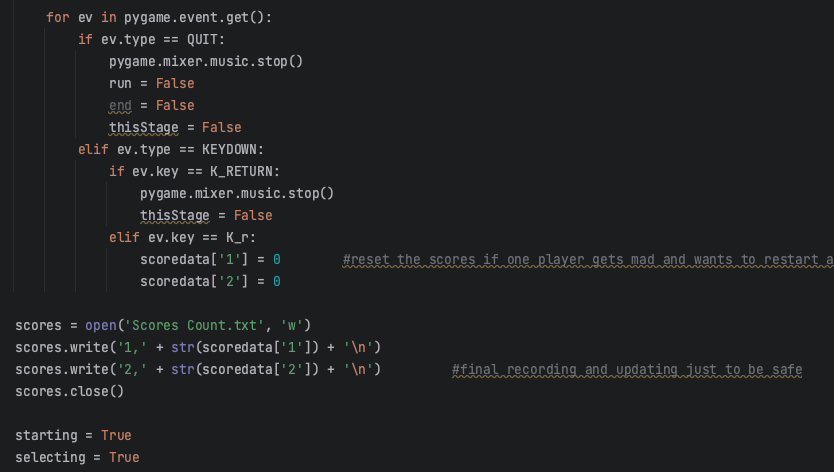
\includegraphics[width=12cm,height=7cm]{kq2.png}

    - Hàm sử dụng một vòng lặp while để liên tục kiểm tra xem màn hình kết thúc trò chơi đang được hiển thị hay không (thisStage là True).
    
    - Trong mỗi lần lặp của vòng lặp này, hàm tạo ra các surface chứa text cho điểm số của người chơi 1 và người chơi 2 sử dụng font đã chỉ định trước và màu sắc cụ thể.
    
    - Các surface này sau đó được xuất (blit) lên màn hình tại vị trí xác định. Cận cảnh của màn hình kết thúc trận đấu, tiêu đề chiến thắng, điểm số, và hướng dẫn cũng được xuất lên màn hình, pygame.display.flip() được gọi để cập nhật toàn bộ màn hình hiển thị với những thay đổi vừa được xuất lên.
    
    - Hàm cũng xử lý sự kiện từ người dùng: Nếu phát hiện sự kiện thoát (QUIT), hàm sẽ dừng phát nhạc nền, cập nhật trạng thái của các biến điều khiển trò chơi (run, starting, selecting), và thoát khỏi vòng lặp while, dẫn đến kết thúc hàm. Nếu phát hiện sự kiện nhấn phím
(KEYDOWN), hàm kiểm tra xem phím được nhấn là phím nào:

    - Nếu phím Enter được nhấn, hàm sẽ dừng phát nhạc nền và thoát khỏi vòng lặp while, có thể là để trở về menu chính của trò chơi & phím R được nhấn, hàm sẽ reset điểm số của người chơi 1 và người chơi 2 về 0.

    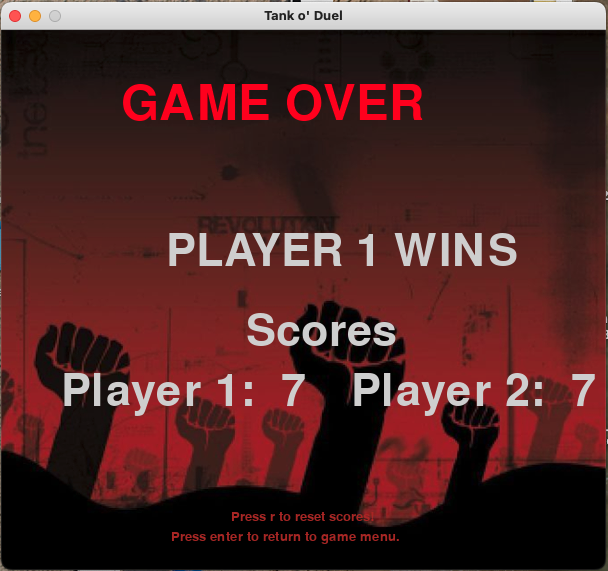
\includegraphics[width=12cm,height=7cm]{imgkq.png}
    

	\section{KẾT LUẬN}
	
	Trong quá trình thực hiện đồ án phát triển phần mềm mã nguồn mở Game tank, nhóm chúng em đã học hỏi được nhiều kỹ năng và kiến thức mới về lập trình, chúng em đã tạo ra một môi trường game thú vị với đồ họa hấp dẫn và âm thanh sống động. Dự án đã giúp chúng ta áp dụng và củng cố kiến thức về lập trình và phát triển game. Việc xây dựng game bắn xe tank không chỉ đòi hỏi kiến thức vững về lập trình mà còn yêu cầu khả năng tư duy logic và sáng tạo trong việc thiết kế gameplay và các tính năng. Tuy nhiên, vẫn còn một số cải tiến có thể thực hiện trong tương lai để nâng cao trải nghiệm của người chơi, bao gồm việc thêm vào các tính năng mới, tối ưu hóa hiệu suất và mở rộng phạm vi gameplay. Nhóm em xin chân thành cảm ơn!

\newpage
%%%%%%%%%%%%%%%%%%%%%%%%%%%%%%%%%
\begin{thebibliography}{80}


\bibitem{Pygame}
Documentation of Pygame ''\textbf{https://www.pygame.org/docs/}''


\end{thebibliography}


\end{document}

